\section{(W) Event Based Avoidance}\label{sec:EventBasedAvoidance}
\begin{itemize}
    \item Introduce the context for Event based avoidance: 
    \begin{itemize}
        \item Preventive DAA - before flight preparation
        \item Event-based DAA - reaction window in minutes, usually cooperative via notifications and other methods
        \item Reactive DAA - you know the drill boys ..., reaction window in 10th of seconds ...
    \end{itemize}
    \item Introduce the process of notification and Event Resolution
    \item Outline hierarchy in U(A)TM controlled space 
    \item Outline expected minimal set of data sources
\end{itemize}

\subsection{(W) Mid-Air Collision Prevention}\label{sec:MidairCollisionPrevention}
\begin{itemize}
    \item Identify and dispute shortcomings of Aircraft classification in ICAO
    \item List of MAC events
    \item For each event describe trigger and resolution 
    \item cite barrel \cite{welzl1991smallest}
\end{itemize}

\subsection{(W) Weather Impact}\label{sec:WeatherImpact}

    \begin{itemize}
        \item do not use term "climate change"
        \item critical events are getting more localized and their magnitude is increased
        \item List of Weather event
        \item Discuss weather mitigation
    \end{itemize}
    
    \emph{Weather Impact} on transportation in general has been introduced by Koetse in study \cite{koetse2009impact}.
    
    \emph{Weather-based} preemptive planning have been introduced into manned aviation in 2015 \cite{yamashita2015climate}. \TBD{This one shows global model impact}
    
    \emph{Severe Weather Condition Detection Capabilities} for current level of standard aviation equipment have been reviewed in \cite{smith2016multi} \TBD{This one shows intermediate weather detection}
    
    \begin{figure}[H]
	\centering
	\begin{subfigure}{0.45\textwidth}
		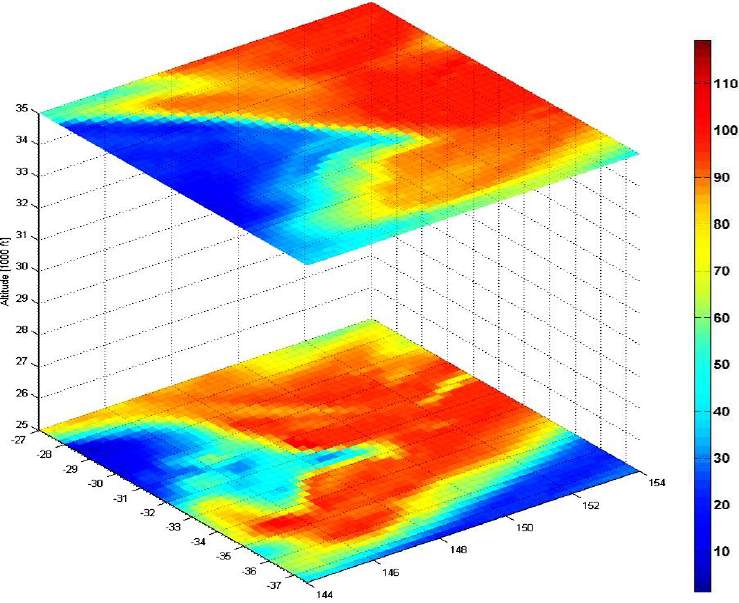
\includegraphics[width=\textwidth]{\FIGDIR/02_03_RelativeHumidity}
		\caption{Relative Humidity.} 
	\end{subfigure}
	\vspace{1em} 
	\begin{subfigure}{0.45\textwidth} % width of right subfigure
		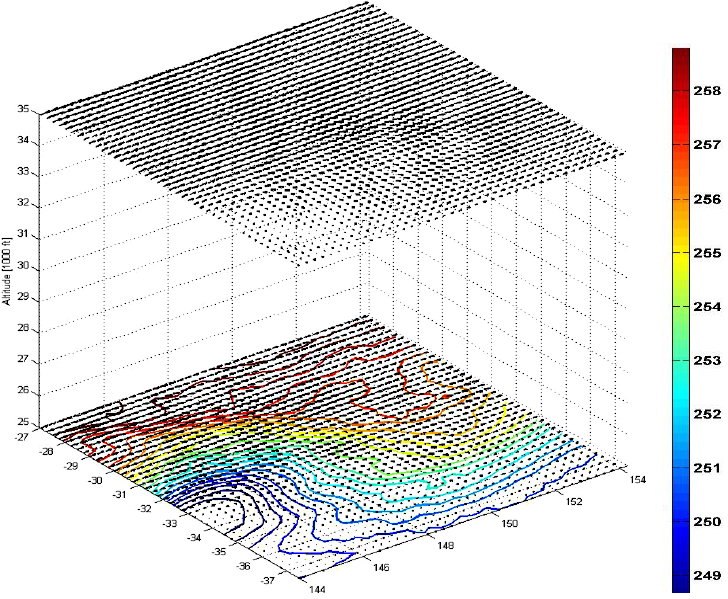
\includegraphics[width=\textwidth]{\FIGDIR/02_04_WindTemperature}
		\caption{Localized Wind Vectors.} % subcaption
	\end{subfigure}
	\caption{Localized Weather Model \cite{balaban2017dynamic}.} % caption for whole figure
    \end{figure}
    
    \emph{Icing risk} in localized environment have been predicted based on numerical model \cite{thompson2017numerical}. It is shown that icing can be prevented by \emph{planned} and \emph{reactive} avoidance.
    
    \emph{Weather Models} can be extracted from \emph{Climate and weather model archive at the National Oceanic and Atmospheric Administration} \cite{rutledge2006nomads}.
    
    \begin{figure}[H]
        \centering
        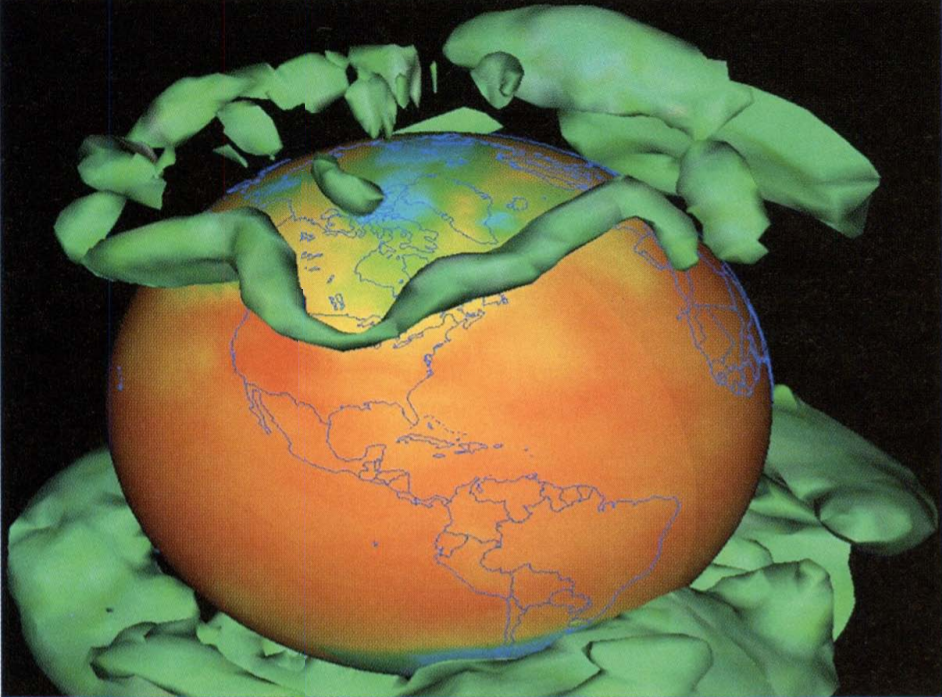
\includegraphics[width=0.7\textwidth]{\FIGDIR/02_01_IVS_Model}
        \caption{Example of upper troposphere winds \cite{rutledge2006nomads}.}
        \label{fig:ExampleOfTroposphereWinds}
    \end{figure}

